When it comes to using $\displaystyle O_{\mathrm{IML}}$
\eqref{eq:iml}, $\displaystyle O_{\mathrm{MML}}$ \eqref{eq:mml}, and
$\displaystyle O_{\mathrm{RER}}$~\eqref{eq:rer} for learning from
sparse feedback (\eg~program synthesis) and comparing the empirical
behavior of these different objective functions, there seems to be
some disagreement among previous work. \citet{pqt2018} suggest that
IML outperforms RER on their program synthesis problem, whereas
\citet{liang2017nsm} assert that RER significantly outperforms IML on
their weakly supervised semantic parsing problem.  Here, we present
some arguments and empirical evidence that justify the results of both
of these papers, which helps us develop a novel combination of IML and
RER that improves the results of \cite{liang2017nsm}.

Inspired by~\cite{norouzi2016reward,nachum2016improving}, we first
note that the IML objective per context $\vx$ can be expressed in
terms of a KL divergence between an optimal policy $\pi^*$ and the
parametric policy $\pi$, \ie~$\kl{\pi^*}{\pi}$, whereas the RER
objective per context $\vx$ can be expressed in terms of the same KL
divergence, but {\em reversed}, \ie~$\kl{\pi}{\pi^*}$. It is well
understood that $\kl{\pi^*}{\pi}$ promotes {\em mode covering}
behavior, whereas $\kl{\pi}{\pi^*}$ promotes mode seeking behavior. In
other words, $\kl{\pi^*}{\pi}$ encourages all of the trajectories in
$\setAp$ to have an equal probability, whereas RER, at least when
$\tau = 0$, is only concerned with the {\em marginal} probability of
successful trajectories and not with the way probability mass is
distributed across $\setAp(\vx)$ (very much like MML).
Notably, \citet{guu2017language} proposed an objective combining RER and MML
to learn a robust policy that can discount spurious trajectories.

Our key intuition is that for the purpose of exploration and
collecting a diverse set of successful trajectories (regardless of
whether they are spurious or not) robust behavior of RER and MML
should be disadvantageous. On the other hand, the mode covering
behavior of IML should encourage more exploratory behavior. We conduct
some experiments to evaluate this intuition, and
in \figref{fig:exploration}, we plot the fraction of contexts for
which $\lvert \setBp(\vx) \rvert \ge k$, \ie~the size of the buffer
$\setBp(\vx)$ after convergence is larger than $k$ as a function of
$k$ on two semantic parsing datasets.

\begin{figure}[t]
  \begin{center}
    \begin{tabular}{@{}c@{}c@{}}
      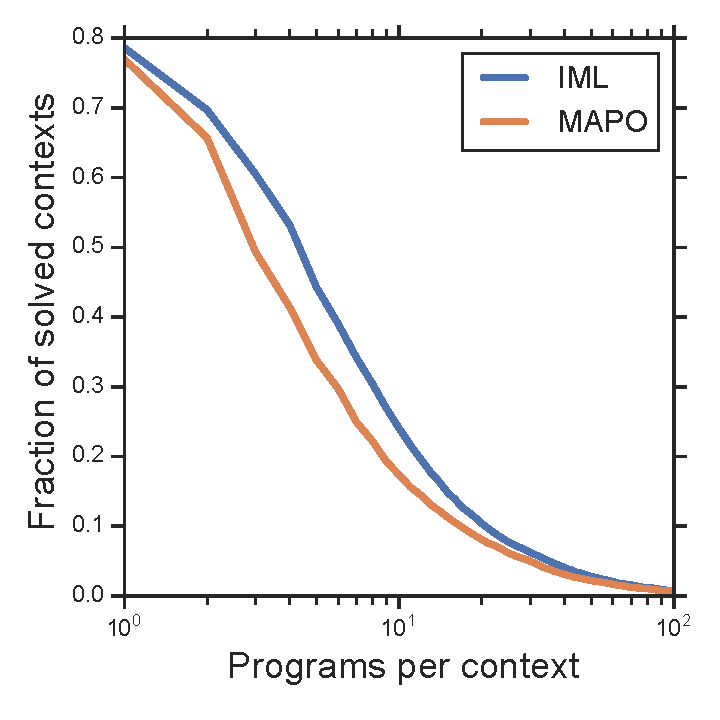
\includegraphics[width=.51\columnwidth]{wtq_iml_mapo} & 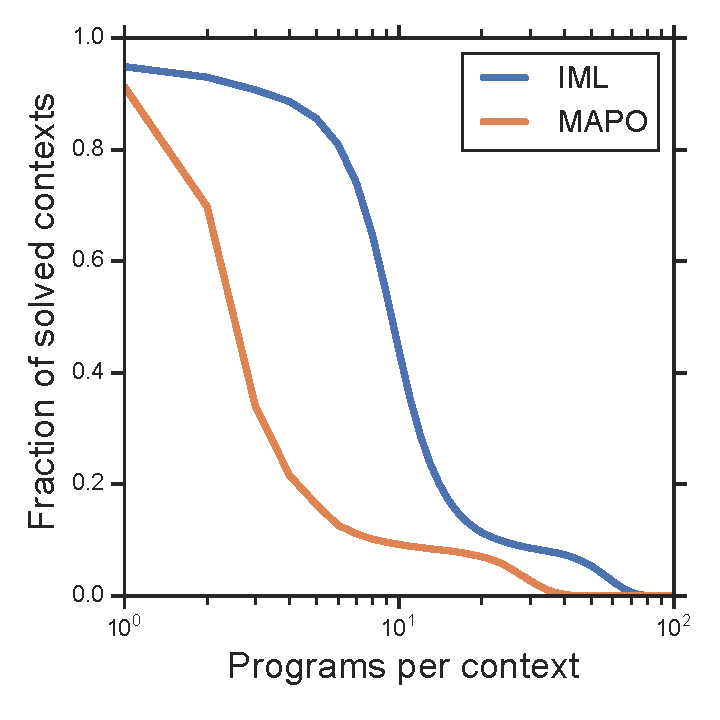
\includegraphics[width=.51\columnwidth]{wikisql_iml_mapo} \\[-.2cm]
      (a) & (b) \\
    \end{tabular}
    % \vspace{-5pt}
    \vspace*{-0.1in}
    \caption{Fraction of total contexts for which at least k programs ($\displaystyle 1 \le k \le 100$) are discovered
    during the entire course of training using the IML and MAPO (\ie~RER)
    objectives on weakly-supervised semantic parsing datasets
    (a) \textsc{WikiTableQuestions} and (b) \textsc{WikiSQL}.
    } \label{fig:mapo_iml_comparison} \end{center}
\label{fig:exploration}
\vspace*{-0.35in}
\end{figure}

Interestingly, we find that IML generally discovers many more
successful trajectories than MAPO. For example, the fraction of
context for which no plausible trajectory is found ($k=10^0$ on the
plots) is reduced by a few percent on both datasets, and for all other
values of $k > 1$, the curve corresponding to IML is above the curve
corresponding to MAPO, especially on \textsc{WikiSQL}. Examining the details of
the experiments in~\citet{pqt2018}, we realize that their program
synthesis tasks are primarily about discovering an individual program
that is consistent with a few input-output examples. In this context,
due to the presence of multiple input-output pairs, the issue of
underspecified rewards poses a less serious challenge as compared to the
issue of exploration. Hence, we believe that the success of IML in that context is
consistent with our results in \figref{fig:exploration}.

Based on these findings, we develop a novel combination of IML and
MAPO, which we call MAPOX (MAPO eXploratory). The key difference
between MAPO and MAPOX is in the way the initial memory buffer of
programs is initialized. In addition to using random search to
populate an initial buffer of programs as in~\cite{NIPS2018_8204},
we also use IML to find a large set of diverse trajectories, which are
passed to MAPO to select from. MAPOX can be interpreted as a two-stage
annealing schedule for temperature in \citet{nachum2016improving}, where one 
would use log-likelihood first ($\infty$ temperature) and then switch to expected
reward (zero temperature). In our experiments, we observe a notable gain from
this form of mode covering exploration combining the benefits of IML and MAPO.\\
